\section{Experimental Setup}
\label{sec:experimentalSetup}
For a fair comparison between the performance of DASH over TCP and QUIC, 
%it is essential to keep network conditions identical for both the protocols. Maintaining identical network condition in a real network is difficult; however, experiments in synthetic network or emulated network may not reflect a real world scenario. So, 
we use an experimental test network as shown in Fig.~\ref{fig:expeirmental_setup}. We use a streaming server to keep all the videos encoded at different video bitrates as mentioned later and a web-based javascript DASH player provided by DASH Industry Foundations (DASHIF)\footnote{\url{https://github.com/Dash-Industry-Forum/dash.js}, (\lastaccessedtoday)} to stream the videos at the client side. To emulate realistic traffic behavior over the test setup, we use a benchmark traffic shaper {\tt Mahimahi}~\cite{mahimahi} and have created {\tt Mahimahi} compatible traces from two publicly available datasets -- (i) a broadband trace from FCC~\cite{dataset-fcc} and (ii) the 3G/HSDPA mobile dataset collected in Norway~\cite{dataset-norway}.
%We have depicted our experimental setup in Fig.~\ref{fig:expeirmental_setup}. As shown in the figure, 

\begin{figure}[h]
	\centering
	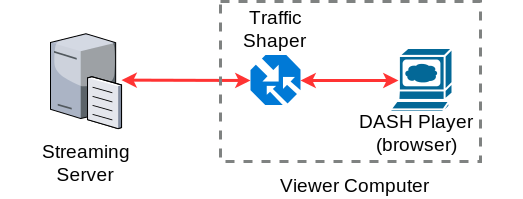
\includegraphics[width=0.8\linewidth]{img/experimental_setup}
	\caption{\label{fig:expeirmental_setup}Experimental setup for video streaming using DASH}
\end{figure}

%\notesc{Give the details of the traffic traces and the traffic shaping method used.}

We run two servers with the different end-to-end data transfer protocols, one for QUIC and another for TCP. For QUIC server, \blue{we use the {\tt golang} implementation of QUIC -- \texttt{GO-QUIC}\footnote{\url{https://github.com/lucas-clemente/quic-go} (\lastaccessedtoday)} (release version 12.0)}. \blue{We have also tested with other QUIC implementations like LiteSpeed QUIC~\footnote{\url{https://github.com/litespeedtech/lsquic} (\lastaccessedtoday)} and have similar observations as reported in this paper. We give the results corresponding to the \texttt{GO-QUIC} implementation as it has been used by majority of the existing works in literature}. For TCP based server, we use the standard {\tt webfsd}\footnote{https://www.gsp.com/cgi-bin/man.cgi?section=1\&topic=webfsd (\lastaccessedtoday)} web-server \blue{(version 1.21)}. As only the {\tt Google Chrome} and the {\tt Chromium} browsers support the QUIC protocol, we use the {\tt Google Chrome} browser \blue{of compatible version 68}, for our experiments to stream the videos at the client side over the DASHIF streaming player.

\blue{
In all the experiments, we use off-the-shelf applications and run them in a non-root user mode. The streaming server and the DASH players run over systems with 8GB of RAM and Intel(R) Core(TM) i5-4590 CPU @ 3.30GHz processor running Ubuntu 16.04.6 LTS operating system on top of Linux 4.9.78. For DASH client, we modify dash.js v2.9.3 to add support for advance ABR algorithms like Pensieve and MPC.
}

\begin{table}[h]
     \caption{\label{table:bitrate}Bitrate and resolution map of DASHified videos.}
	\centering
	\begin{tabular}{|l|c|c|c|c|}
		\hline
		Bitrate(kbps) & 200 & 400 & 600 & 800 \\ \hline
		Resolution & 320x180 & 320x180 & 480x270 & 640x360 \\ \hline \hline
		Bitrate(kbps) & 1000 & 1500 & 2500 & 4000 \\ \hline
		Resolution & 640x360 & 768x432 & 1024x576 & 1280x720 \\ \hline
	\end{tabular}
\end{table}

We use a total of $45$ hours of videos (about $50$ different videos) which have been dashified (encoded in different bitrates as shown in Table~\ref{table:bitrate}) using the {\tt ffmpeg} tool in eight different video quality levels and two different audio quality levels. \blue{We play every videos for all the ABRs and protocol combinations, resulting $\approx 19$ days of video playback time. We also maintain the similar playback environment for DASH/QUIC and DASH/TCP for each of the video and the ABR combinations.} 
%During the playback, we collect all the relevant data like the buffer occupancy, the measured bandwidth, the current playback quality and other video QoE statistics. We have compared multiple QoE parameters like the video startup delay, the rebuffering time and the playback smoothness of the videos. Further, 
We have compared the performance across five different ABR mechanisms, namely, BOLA (B)~\cite{bola-2016}, the standard buffer-based quality adaptation of DASHIF (BB), the two variants of model predictive control (MPC) driven approaches~\cite{yin2015control} -- MPC\blue{-Fast} (MF) and MPC\blue{-Robust} (MR) and the deep learning driven quality adaptation algorithm -- Pensieve (P)~\cite{mao2017neural}. To measure the overall QoE of the video playback, we have used a combined metric of the average quality level, the rebuffering time and the playback smoothness, as used in~\cite{yin2015control,mao2017neural}.
\begin{equation}
QoE=\sum_{n=1}^{N}q(R_n)-\mu\sum_{n=1}^{N}T_n-\sum_{n=1}^{N\blue{-1}} \bigg\vert q(R_{n+1})-q(R_n)  \bigg\vert
\label{eqn:QoE}
\end{equation}
%\label{para:eqnexp}
Eq.~(\ref{eqn:QoE}) indicates the QoE metric to measure the overall QoE of a video playback session. Here, $N$ is the total number of chunks for the playback video. $R_n$ and $q(R_n)$ are the representation of the playback bitrate of the chunk $n$ and the quality perceived by a user for that chunk $n$. $T_n$ is the rebuffering time for the chunk $n$. $\mu$ is a QoE weight factor \cite{yin2015control}. 
%Now, $q(R_n)$ has been used differently at different literature depending on the user perceived priority on the video playback instances. 
We consider a linear representation $q(R_n) = R_n$, similar to~\cite{yin2015control}, indicating that the playback quality increases linearly with the increase of playback bitrate. 
%
%Two popular representations of $q(R_n)$ are as follows.
%\begin{enumerate}
%	\item $QoE_{lin}$: $q(R_n) = R_n$~\cite{mpc:2015}: \notesc{Give the meaning of this equation}\noteam{Already mentioned in the paragraph \ref{para:eqnexp}}.
%	\item $QoE_{log}$: $q(R_n) = \log(R/R_{min})$~\cite{bola-2016}. \notesc{Give the meaning of this equation}.
%\end{enumerate}
%\notesc{Have you shown the results for both the metrics?}\noteam{Previously I shown results for both. Currently I not. However, I can calculate it.}

